\documentclass[12pt, conference, compsoc, onecolumn]{IEEEtran}
\usepackage{graphicx}
\usepackage{listings}
\usepackage{amsmath}
\usepackage{amssymb} % For \mathbb and other symbols
\usepackage{array, float}
\usepackage[colorlinks=true]{hyperref}
\usepackage[style=numeric,backend=bibtex]{biblatex}
\graphicspath{ {./figures/} }
\addbibresource{refs.bib}

\lstdefinestyle{model_arch}{
	backgroundcolor=\color{white},   
	basicstyle=\ttfamily,
	breaklines=true,
	showstringspaces=false,
	frame=single, % This adds a box around all sides of the snippet
	rulecolor=\color{black}, % You can specify the color of the box
}

\begin{document}
	\title{ECE1512 - Digital Image Processing and Applications - Project B}
	\author{Swapnil Patel - 999728870 - \today}
	
	\author{\IEEEauthorblockN{Swapnil Patel}
		\IEEEauthorblockA{
			University of Toronto\\
			swap.patel@mail.utoronto.ca\\
			Code: \href{https://github.com/Swapnil949/ECE1512\_2024F\_ProjectRepo\_SwapnilPatel}{Swapnil949/ECE1512\_2024F\_ProjectRepo\_SwapnilPatel}
	}}
	
	\maketitle
	
	\section{Vision Language Models (VLMs) - LLaVA: Large Language and Vision Assistant}
	
	In this section, LLaVA (Large Language and Vision Assistant), as presented in the paper "Visual Instruction Tuning" \cite{liu2023llava}, is discussed. LLaVA is an end-to-end trained multimodal AI system that connects a vision encoder with a large language model (LLM) to interpret and follow human instructions involving both visual and linguistic contexts. The work in this paper represents the first attempt to use language-only GPT-4 to generate multimodal language-image instruction-following data, enabling instruction tuning for multimodal tasks.
	
	The paper demonstrates that LLaVA achieves remarkable capabilities in multimodal chat, often exhibiting behaviors similar to multimodal GPT-4 on unseen images and instructions. Evaluations show an 85.1\% relative score compared to GPT-4 on a synthetic multimodal instruction-following dataset. Furthermore, when fine-tuned on ScienceQA, LLaVA achieves a new state-of-the-art accuracy of 92.53\%, highlighting its effectiveness in reasoning and answering visual and textual queries. To facilitate further research, the authors release the GPT-4-generated visual instruction tuning data, their model, and associated codebase to the public.
	
	\subsection{LLaVA Architecture}
	\begin{figure}[H]
		\centering
		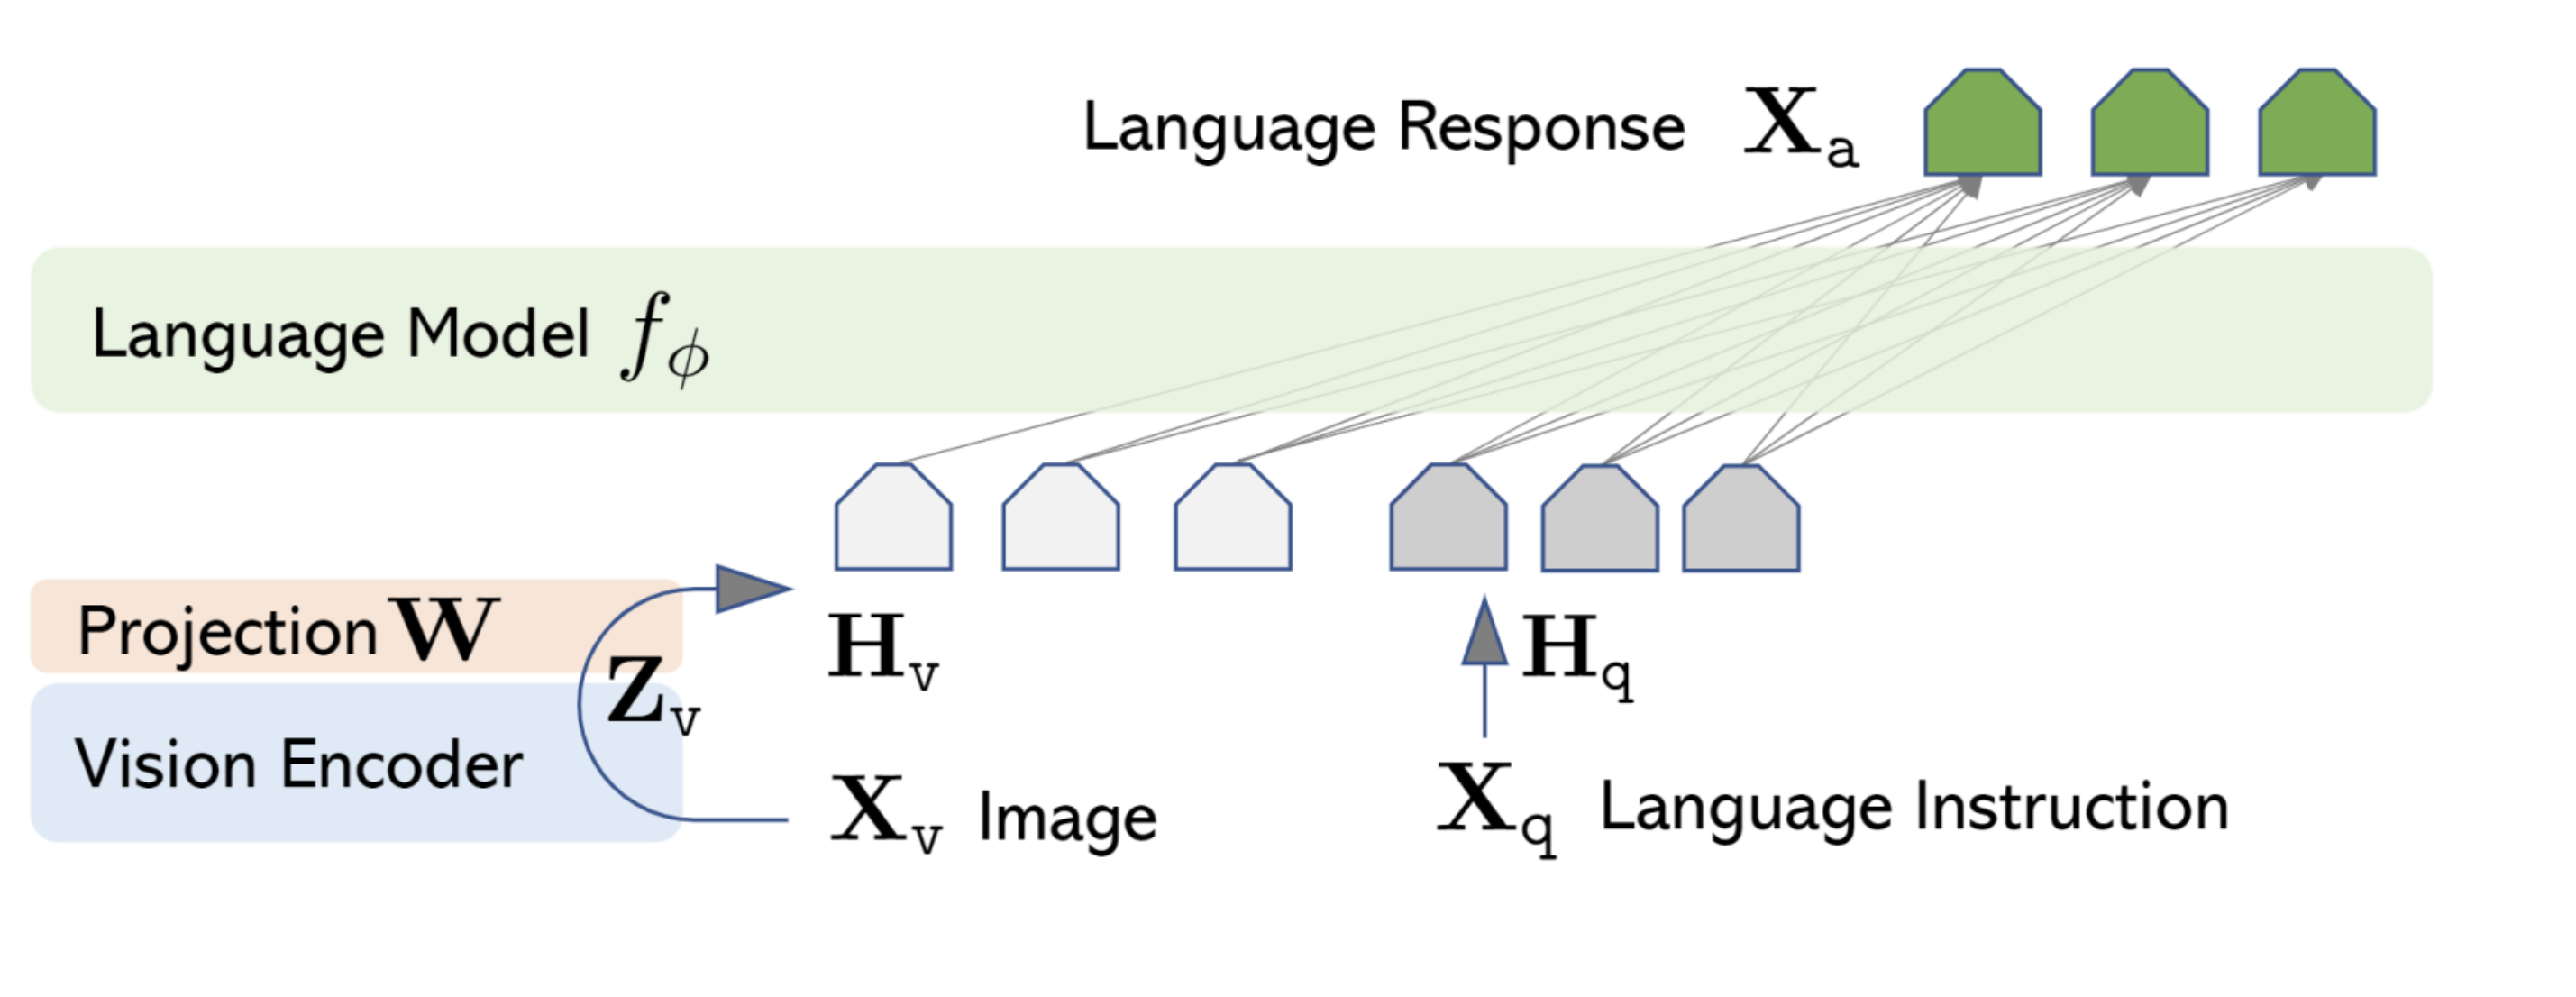
\includegraphics[width=0.75\textwidth]{figures/conceptual-diagram-of-llava.png}
		\caption{LLaVA Architecture \cite{liu2023llava}}
		\label{fig:llava_arch}
	\end{figure}
	
	The LLaVA (Large Language and Vision Assistant) model architecture is designed to integrate visual and linguistic modalities to enable advanced multimodal understanding. Its structure consists of several key components, which work together to process both image and text inputs, generating coherent and context-aware responses.
	\subsubsection*{Vision Encoder} 
	At the foundation of the architecture is the Vision Encoder, which processes the input image $X_v$. This encoder (e.g., CLIP) transforms the raw image data into a high-dimensional feature representation $H_v$. These features encapsulate the visual information in a format suitable for downstream processing.
	
	\subsubsection*{Projection Layer} 
	The Projection Layer serves as a critical bridge between the Vision Encoder and the Language Model. It applies a projection matrix $W$ to convert the feature representations $H_v$ into a format $Z_v$ that is compatible with the language model's embedding space. This alignment ensures seamless integration of visual data with textual data for joint processing.
	
	\subsubsection*{Language Instruction Input}
	Alongside the visual input, the model receives a Language Instruction input $X_q$, which represents the textual task or query. This input is processed by the language model to generate its own feature representation $H_q$, encapsulating the semantic meaning of the query.
	
	\subsubsection*{Language Model}
	At the core of the architecture is the Language Model $f_\phi$, which is a pre-trained large language model (e.g., Vicuna). This model takes both the projected visual features $Z_v$ and the linguistic features $H_q$ as input, integrating them to produce a unified understanding of the multimodal context.
	
	\subsubsection*{Output Generation}
	The final output, $X_a$, is a language-based response that incorporates information from both the visual and textual inputs. This response can range from answering specific questions about an image to providing detailed descriptions or engaging in complex reasoning tasks that require a multimodal perspective.
	
	\subsection{LLaVA Shortcomings}
	\subsubsection*{Limited Contextual Understanding of Images}
	\hfill\\
	LLaVA relies on pre-trained vision encoders, such as CLIP, for image feature extraction. While these encoders perform well on general tasks, they often fail to capture fine-grained details or spatial relationships within images. This limitation affects tasks requiring detailed visual reasoning, such as understanding complex scenes, interpreting object interactions, or recognizing small or subtle objects. For instance, in an image with overlapping objects, LLaVA might struggle to disentangle the spatial layout or distinguish individual components accurately.
	\subsubsection*{Suboptimal Fusion of Vision and Language Modalities}
	\hfill\\
	The integration of visual and textual features in LLaVA's architecture is not fully optimized for complex relationships. Current fusion mechanisms may inadequately align the visual embeddings with language tokens, leading to subpar reasoning when tasks demand intricate multimodal understanding. For example, in visual dialogue tasks or when resolving referring expressions (e.g., identifying "the cat on the left next to the sofa"), the model might misinterpret the contextual alignment or fail to generate coherent responses
	\subsubsection*{Inability to Reason Over Temporal Dynamics}
	LLaVA is primarily designed for static image understanding and does not support sequential or temporal inputs like videos. This limitation prevents it from handling tasks that require reasoning over changes in a scene or understanding temporal dependencies, such as action recognition or video-based question answering. For instance, in a video of a ball rolling off a table, LLaVA cannot infer causal relationships or describe the sequence of events due to its lack of temporal modeling capabilities.
	
	\hfill\\
	Above mentioned issues, contribute to redundant computations, increased memory usage, and latency during both training and inference. As a result, the model struggles to achieve optimal performance without incurring high computational costs, making it less scalable and efficient for real-world multimodal applications. Addressing these challenges is critical to reducing the computational overhead and unlocking the full potential of LLaVA.
	
	\subsection{Cobra}
	
	To address some of the issues with LLaVA, Cobra \cite{zhao2024cobraextendingmambamultimodal} was introduced by Zhao et al. It is designed to enhance the efficiency and performance of LLMs especially for multimodal tasks. It integrates the Mamba language model with visual modalities, extending its computational benefits to include visual processing. The key innovation of Cobra is its ability to reduce the computational complexity from quadratic (like traditional Transformer networks) to linear, making it more efficient for handling multimodal inputs. This efficiency is achieved through Mamba’s linear sequential modeling, which allows Cobra to maintain high accuracy while speeding up both training and inference times.
	
	\begin{figure}[H]
		\centering
		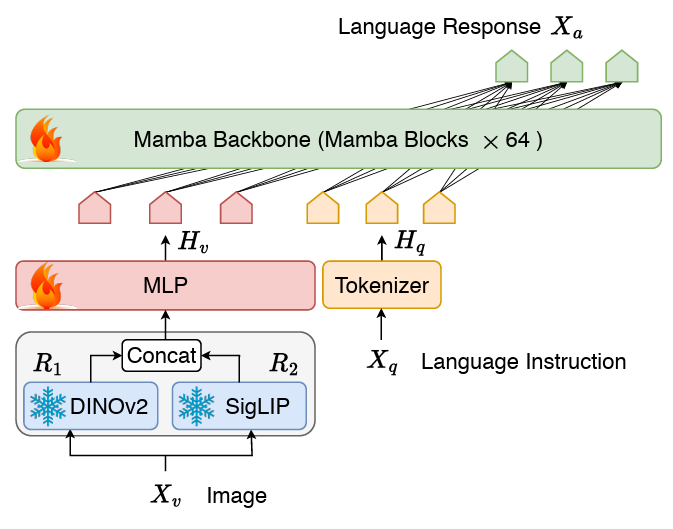
\includegraphics[width=0.55\textwidth]{figures/cobra.png}
		\caption{Cobra Architecture \cite{zhao2024cobraextendingmambamultimodal}}
		\label{fig:cobra_arch}
	\end{figure}
	
	Figure \ref{fig:cobra_arch} shows the model architecture for Cobra. It consists of three key components: a vision encoder, a projector, and a Mamba backbone. The vision encoder merges visual representations from DINOv2 and SigLIP, capturing both low-level spatial properties and semantic details to enhance performance on downstream tasks. The projector aligns these visual features with the text embeddings, either through a multiple-layer perceptron or a lightweight downsample projector to reduce computation. The Mamba backbone, a stack of 64 basic blocks with residual connections and RMSNorm, integrates these multimodal inputs into a unified representation. It processes the concatenated visual and textual embeddings autoregressively to generate natural language outputs. This design enables Cobra to efficiently handle complex multimodal tasks, such as spatial reasoning and visual illusions, with reduced parameter counts and linear computational complexity.
	
	The authors of Cobra demonstrated that their model achieved competitive performance across multiple benchmarks despite having approximately 43\% fewer parameters than LLaVA v1.5 (7B). Cobra outperformed all listed models on the VSR benchmark and most models on VizWiz and POPE, with only Prism performing better. When compared to models with a similar number of parameters, Cobra consistently outperformed LLaVA-Phi across VQAv2, VizWiz, and POPE. Additionally, it showed strong performance on GQA and VQAv2, and was more effective than TinyLLaVA on POPE. These results indicate that Cobra can match the performance of state-of-the-art models of similar size (3B parameters) and remains competitive against larger-scale models (7B and above).
	
	\subsection{Proposed Integration with MambaVision}
	
	To enhance the LLaVA and extend the work done in Cobra, I propose extending its architecture by leveraging the strengths of the MambaVision as the vision encoders. Cobra already showcases the advantages of using Mamba model as the language model backbone. Specifically, we will freeze the Mamba backbone and other layers to maintain compatibility with the LLaVA architecture, ensuring continuity with existing multimodal tasks. Vision Encoder block will be replaced by MambaVision block.
	
	MambaVision is an extension of the Mamba architecture designed to handle visual inputs more effectively. It combines advanced visual feature extraction techniques with the computational efficiency of the Mamba model. MambaVision integrates robust vision encoders that can capture fine-grained spatial details and semantic relationships in images, making it well-suited for tasks that require detailed visual reasoning and understanding of temporal dynamics. 
	
	By utilizing MambaVision as vision encoders, we can take advantage of their robust feature extraction capabilities, which capture detailed visual information and spatial relationships more effectively than traditional vision encoders. 
	
	The proposed LLaVA framework that includes MambaVision is showed below in Figure \ref{fig:llava_update}.
	
	However, due to time and resource constraints, integrating a new vision encoder into LLaVA using MambaVision is beyond the scope of this project. This aspect of the work is proposed as future work, aiming to further extend the work done in Cobra to fully utilize Mamba as the backbone for all foundation models in LLaVA.
	
	\begin{figure}[H]
		\centering
		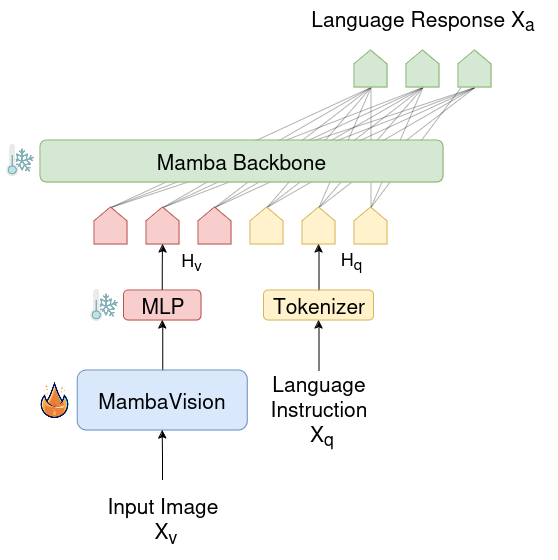
\includegraphics[width=0.55\textwidth]{figures/llava_update.png}
		\caption{Proposed MambaVision Integration to LLaVA and Cobra}
		\label{fig:llava_update}
	\end{figure}
	
	
	\section*{References}
	\addcontentsline{toc}{section}{\protect\numberline{}References}
	\printbibliography[heading=none]
	
	%	\onecolumn
	%	\section*{Appendix}
	%	\addcontentsline{toc}{section}{\protect\numberline{}Appendix}
	
	
\end{document}